%!TEX root = CS_ORNs.tex


%%%%%%%%%%%%%%%%%%%%%%%%%%%%%%%%%%%%%%%%%%%%%%%%%%%%%%%%%%%%%%%%%
%%%%%%%%%%%%    		INTRODUCTION	    		%%%%%%%%%%%%%
%%%%%%%%%%%%%%%%%%%%%%%%%%%%%%%%%%%%%%%%%%%%%%%%%%%%%%%%%%%%%%%%%

Animals identify and discriminate odors using olfactory receptors (Ors) expressed in olfactory receptor neurons (ORNs)~\cite{Or_ORNs_maps, buck1991novel}. In both insects and vertebrates, distinct ORNs, which typically express a single Or, respond broadly to many distinct volatile odorants~\cite{malnic1999combinatorial, mosquito_combinatorial_coding, hildebrand1997mechanisms, hallem_carlson, debryune_odor_coding, friedrich1997combinatorial}. Likewise, any given odorant may incite strong responses in a number of ORNs. ORN tuning curves are therefore broad and overlapping, implying that odors are encoded combinatorially -- by the particular combination of responses they elicit in the ORN repertoire, patterns which are eventually decoded downstream into behavioral response~\cite{early_olfactory_processing}.


%The number of odors that humans can discriminate is large, at least tens of thousands (but possibly trillions), far greater than the number of functional ORs we express. The same disparity holds true for \textit{Drosophila}, and it has been suggested that accurate combinatorial coding of a high-dimensional odor signal via a low-dimensional receptor space may be possible by exploiting a)~the fact that most natural odors are sparse in their volatile molecular constituents (ex.) and b)~ORN responses to these volatile molecules are broad and random. These two features permit accurate reconstruction of a large number of complex odors from a limited OR repertoire. Downstream circuitry may further support this paradigm. In \textit{Drosophila}, ORNs synapse onto glomeruli in the antennal lobe (AL), where they then diverge randomly onto Kenyon cells in the mushroom body (MB)~\cite{early_olfactory_processing, abbott_axel}. %Signals in the MB are sent to higher order brain centers and decoded into behavioral response~\cite{olfactory_map_chiang, mushroom_body_review}. Within a framework of combinatorial decoding of sparse signals, the expansive synaptic connections from AL to MB~\cite{abbott_axel} may play a key role in learning and robust odor discrimination~\cite{vijay_1}.



%The efficacy of combinatorial coding hinges on simultaneously relaying odor identity and intensity within an ensemble of neural response. In addition to passing information through response combinatorics (across neurons), this strategy may also exploit response dynamics (across time). In locust projection neurons (PNs), for example, both identity- and intensity-relevant information is separately encoded within the temporal firing patterns of the PN population. It has also been shown that temporal responses across neuron populations can resolve stimuli reliably, despite potentially conflicting dynamics in the stimulus itself~\cite{brown2005}. Further, the breadth of OR sensitivities to a particular odorant implies that ORNs will be activated in a unique order to any given odor. Odor identity could thus be encoded by either by the temporal sequence of ORN recruitment, or by the subset of earliest responders. {\color{blue} Say something more about primacy coding.}

Odor signals in nature are uniquely complex in composition, space, and time, and like other sensory modalities, olfactory systems must tune their response to the character of input stimuli~\cite{murlis_odor_plumes, fluid_dynamics_chemosensory, celani, carde_navigation, srinivas_elife}. Various features of natural odor signals are power-law distributed, producing whiffs of widely varying duration and intensity~\cite{celani}. Sensitivity to low concentrations could thus lead to saturation at high intensities, confounding combinatorial representations of odor identity. Further, ethologically-relevant odors are often mixed together with nuisance odors; due to the non-specificity of ORN response, distinct odors could simultaneously activate overlapping ORN subsets, preventing  accurate disambiguation~\cite{odor_backgrounds}. 

What invariances and adaptive mechanisms %in the olfactory pathway 
might help preserve combinatorial odor representations in natural environments? 
%As low odorant concentrations can activate even a single receptor, then 
%representation by either the sequence of activated receptors or the subset of earliest responders could fluctuate rapidly. THIS is wrong.
%{\color{blue} Say something about different numbers of ORNs getting recruited}. Further, ethologically-relevant odors are often mixed together with nuisance backgrounds. %Other sensory systems adapt response characteristics, such as gain and sensitivity, in order to maintain coding accuracy in changing environments.
%Several recent studies have uncovered invariances and adaptive mechanisms in the \textit{Drosophila} olfactory sensing periphery that {\color {blue} Say how the invariances refer to single ORN but not known how it affects combinatorics?}
In \textit{Drosophila} larvae, dose responses of 324 OR-odorant combinations obey a single activation function shape, with similar Hill coefficients but different activation thresholds, which are distributed as a power law~\cite{si2017invariances}. \textit{Drosophila} ORNs also exhibit a large degree of similarity in their temporal integration of fluctuating stimuli. While for some Or-odor combinations, ORN response can exhibit large differences, such as super-sustained responses~\cite{montague2011similar}, deconvolution of stimulus dynamics from neuron responses produces stereotyped filters that differ little among ORNs~\cite{martelli}. %5Larval ORNs have also been shown to exhibit a single temporal integration filter~\cite{si2017invariances}. 

Beyond these invariances are adaptive mechanisms which can preserve odor representations amid environmental changes.
In \textit{Drosophila}, antennal lobe glomeruli receiving connections from ORNs send mutually inhibitory connections, effectively normalizing incoming ORN signals before they are projected to the lateral horn and mushroom body~\cite{lateral_inh_asahina, divisive_normalization}. In the mushroom body, inhibition from giant interneuron upon Kenyon cells further acts to suppress  patterns of activity elicited by these odors~\cite{giant_inhibitory_neuron}. Further, upstream of these connectivity-mediated mechanisms, individual ORNs themselves adapt in time an apparently universal way: ORN gain varies inversely with mean odor concentration according to Weber's Law of psychophysics~\cite{weber1996eh}, while maintaining response time independent of odor intensity~\cite{srinivas_elife,cafaro_WL, cao_WL}. Weber's Law has been observed in several OR-odorant combinations, and is traced to feedback mechanisms operating at the level of odor transduction, upstream of ORN firing machinery~\cite{srinivas_elife}. This points to a mechanistic origin involving modification of phosphorlyation sites on the universal \textit{Drosophila} co-receptor Orco.  Other phosphorylation sites on Orco have been implicated in desensitization to odors over longer timescales as well~\cite{Guo_Smith_review,Guo_Smith}.  

While in a single channel system such as \textit{E. coli}, adaptive feedback via Weber's Law is known to robustly maintain sensitivity in response to mean concentration changes, the implications for a multiple-channel system -- which combines information from several sensors with overlapping receptive fields  -- is less straightforward. Here we combine a biophysical model of universal ORN adaptive response and neural firing with various sparse signal decoding frameworks to explore whether and how ORN adaptation maintains accurate combinatorial coding of odor signals that span varying degrees of intensity, molecular complexity, and temporal structure. 
%in natural environments. 
%As combinatorial coding relies fundamentally on responses being sufficiently dispersed in OR space, it is vulnerable to effects that reduce sparsity. For example a sudden increase in  odor intensity, not atypical in natural environments~\cite{celani}, increases the number of ORs that respond and can saturate some of them\cite{kajiya2001molecular,wang2003two,hallem_carlson}. Likewise, the presence of background odors may activate additional ORs.  
%Some of this reduction of coding capacity in the OR space may be compensated by temporal information in the OR responses to code both stimulus identity and intensity~\cite{friedrich1997combinatorial,intensity_vs_identity,junek2010olfactory,smear2011perception}. 
%Individual ORNs, which typically express only one OR each~\cite{buck1991novel}, respond to many odorants, and individual odorants activate many ORNs~\cite{friedrich1997combinatorial,hallem_carlson,mosquito_combinatorial_coding,nara2011large}. Individual odors are  believed to be combinatorially coded in the distinct patterns of activation they elicit in the olfactory periphery of insects and vertebrates~\cite{hildebrand1997mechanisms,malnic1999combinatorial,laurent2001odor,kajiya2001molecular,wang2003two,kreher2005molecular,junek2010olfactory,smear2011perception}, which are then decoded by downstream circuitry to direct behavior. 
%Recent studies have revealed several invariance in ORN response dynamics that may contribute to robust combinatorial coding. In \textit{Drosophila melanogaster} flies~\cite{hallem_carlson,srinivas_elife} and larvae~\cite{si2017invariances}, the dose responses of various OR-odorant combinations exhibit similar Hill coefficients but different activation thresholds (EC50), which are distributed as a power law~\cite{si2017invariances}. While for some OR-odor combinations ORN response can exhibit large differences such as supersustained responses~\cite{montague2011similar}, Deconvolution of stimulus dynamics from ORN responses for various ORNs in adult flies resulted in stereotyped filters that did not differ much among many ORNs and could predict the response of one ORN to multiple odorants. Similarity among ORN filters was recently demonstrated for the entire ensemble of ORNs in \textit{Drosophila} larvae ~\cite{si2017invariances}. 
%ORN gain in adult flies has been shown to scale inversely with mean odor concentration~\cite{srinivas_elife,cao_WL}, according to Weber-Fechner law~\cite{weber1996eh,fechner2012elemente}, while maintaining response time independent of signal intensity~\cite{martelli,srinivas_elife}. Importantly for odor coding, this observed scaling law was obeyed by many OR-odorant combinations tested. Similarly in larvae, the ORN filters were found invariant with respect to odor intensity\cite{si2017invariances}. Together with the power-law distribution of activation thresholds measured in larvae, this suggests that \textit{Drosophila} ORNs respond to relative changes in odor intensity. This fast adaptation has been traced back to feedback mechanisms taking place at the level of odor transduction, upstream of the ORN firing machinery~\cite{nagel_wilson_biophysical,cao_WL,cafaro_WL,srinivas_elife}, pointing to a mechanistic origin involving modification of phosphorylation sites on the universal co-receptor Orco~\cite{Orco,getahun2013insect,getahun2016intracellular}. Other phosphorylation sites on Orco have been implicated in desensitization to odors over longer timescales as well~\cite{Guo_Smith_review,Guo_Smith}. Finally, in addition to front-end adaptation, normalization enacted through lateral inhibition in the AL may act as a mechanism of gain control further downstream~\cite{divisive_normalization}.
%In nature, relevant odorants are typically mixed with background odorants that can potentially confound odor recognition.  While the adaptive mechanisms just described have been shown to facilitate the tracking of fluctuations in the intensity of monomolecular odorants, we know very little about how adaptation shapes combinatorial coding strategies, whose potential derives not just from the ability to identify single odorants but to discriminate many complex odor signals using a limited OR repertoire. 
We find that front-end gain modulation helps preserve coding capacity within the non-specifically sensing ORN repertoire, and maintains abstract representations of odor identity across different intensities. As such, this adaptive mechanism promotes the  accurate  discrimination of weak odor signals from strong backgrounds of varying molecular complexity, both in static odor environments  and in fluctuating ones. We also investigate the predictions of our model for the \textit{primacy coding} hypothesis  -- that odors are encoded entirely by the subset of a few earliest responding ORNs~\cite{primacy_coding, primacy_math}. Our results agree with primacy coding when odor signals are sufficiently  simple, though signals composed of more molecular constituents require the recruitment of the full ORN repertoire. Finally, we show that front-end adaptation acts in concert with divisive normalization in the antennal lobe to maintain the invariance of activity patterns  in the  mushroom body. Together, our results suggest that despite the broad overlap of ORN tuning curves, a universal mechanism of front-end adaptation may play a vital role in preserving representations of odor identity in naturalistic odor landscapes.



\section{Results}



%%%%%%%%%%%%%%%%%%%%%%%%%%%%%%%%%%%%%%%%%%%%%%%%%%%%%%%%%%%%%%%%%
%%%%%%%%%%%%    		MODEL DESCRIPTION    		%%%%%%%%%%%%%
%%%%%%%%%%%%%%%%%%%%%%%%%%%%%%%%%%%%%%%%%%%%%%%%%%%%%%%%%%%%%%%%%



\subsection{Model of ORN sensing repertoire}



%%%%%%%%%%%%		TUNING CURVES FIGURE			%%%%%%%%%%%%%

\begin{figure*}[!tb]
	\centering
	\begin{subfigure}[t]{\linewidth}
		\phantomsubcaption
		\label{fig:tuning_curves_a}
	\end{subfigure}
	\begin{subfigure}[t]{0\linewidth}
		\phantomsubcaption
		\label{fig:tuning_curves_b}
	\end{subfigure}
	\begin{subfigure}[t]{0\linewidth}
		\phantomsubcaption
		\label{fig:tuning_curves_c}
	\end{subfigure}
	\begin{subfigure}[t]{0\linewidth}
		\phantomsubcaption
		\label{fig:tuning_curves_d}
	\end{subfigure}
	\begin{subfigure}[t]{0\linewidth}
		\phantomsubcaption
		\label{fig:tuning_curves_e}
	\end{subfigure}
	\begin{subfigure}[t]{0\linewidth}
		\phantomsubcaption
		\label{fig:tuning_curves_f}
	\end{subfigure}
	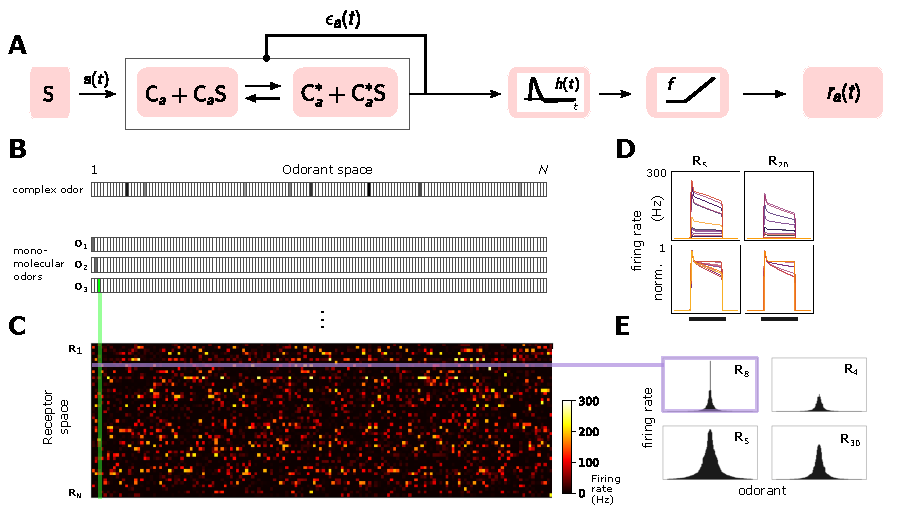
\includegraphics[width=\textwidth]{figures/1_tuning_curves}
	\caption{\footnotesize{
		\textbf{A}~Odor binding model. Or/Orco complexes $\textup{C}_a$ bind odorant molecules $s_i$ comprising stimuli $\textup{S}$. These complexes can stochastically switch between inactive and active states, where the steady-state active fraction is determined by the complex free energy $\epsilon_a(t)$. The activity feeds back on to the free energies with timescale $\tau_a$ to pull the activity to a baseline level $A_{a0}$. ORN firing rates $r_a(t)$ are generated by passing $A_a(t)$ through a linear temporal filter $h(t)$ and a nonlinear thresholding function$f$. 
		\textbf{B}~Odor mixtures are represented by real-valued $N$-dimensional vectors $\mathbf s$, whose components $s_i$ are the concentrations of  the individual molecular constituents  of $\mathbf s$. 
		\textbf{C}~Following (), active binding constants are distributed as a power-law with coefficient $\alpha=0.35$
		\textbf{D}~The maximal firing response of 50 ORNs to the 150-possible monomolecular odors $\mathbf s = s_i$, for the power-law $K^*_{ai}$ distribution in C.
		\textbf{E}~Representative ORN tuning curves, generated by ordering the responses within a single row of the response matrix in D. A diversity of response, mimicking that of~\cite{hallem_carlson}, arises from both the distribution of odorant binding constants $K^*_{ai}$ and the distribution of receptor free energies $\epsilon_a$.}}
		\label{fig:tuning_curves}
\end{figure*}

Odor identification consists of encoding in the sensing periphery followed by decoding in higher-level processing centers of the olfactory circuit. We first examine how front-end adaptation can maintain odor encoding capacity,  by  drawing upon a model of odor-to-ORN firing recently shown to reproduce experimental findings: Weber-Fechner scaling, signal transduction kinetics, and firing rate dynamics of individual \textit{Drosophila} ORNs to fluctuating stimuli ~\cite{srinivas_elife}. Here we generalize this model to a repertoire of $M=50$ ORN types. ORNs house olfactory receptor complexes $\textup{C}_a$, $a=1,...,M$, each consisting of an ORN-specific OR and the universally-expressed olfactory co-receptor Orco, which mediates odor transduction through dendritic localization of and heteromerization with ORs (Fig.~\ref{fig:tuning_curves_a}). These odorant-response functional units interact with odor mixtures, each of which is composed of some combination of $N$ odorant molecules with time-dependent concentrations $s_i(t)$, $i=1,...,N$ (Fig.~\ref{fig:tuning_curves_b}). We choose $N=150$, as this number is sufficiently larger than the size of the sensing repertoire~$M$. Functionally, $\textup{C}_a$ forms a non-selective cation channel whose current is mediated by the strength and nature of bound ligands. We thus model a given complex as stochastically switching between active (channels open) and inactive states, while also being bound or unbound with odorant $i$. The active conformation binds odorant $i$ with higher affinity than the inactive conformation, resulting in distinct dissociation constants, $K^*_{ia}$ and $K_{ia}$, respectively. In steady state, the active fraction $A_a$ of Or/Orco complexes in ORN $a$ can be solved for as (see Methods):
\begin{align}
A_a(t) &= \left(1 + e^{\epsilon_a(t)}\right)^{-1} \nonumber \\
\epsilon_a(t) &= \epsilon_{a, \textup{act}}(t) + \epsilon_{a, \textup{ligand}}(t) \nonumber \\
\epsilon_{a, \textup{ligand}}(t) &= \frac{1 + \sum_i^N s_i(t)/K_{ai}}{1 + \sum_i^N s_i(t)/K^*_{ai}},
\label{eq:steady_state_act_OR}
\end{align}
where $\epsilon_{a, \textup{act}}(t)$ is the free energy cost of $\textup{C}_a$ activation.

Inward currents elicited by activation of the Or/Orco receptor complexes then incite firing activity in ORNs. Following~\cite{srinivas_elife}, we model the Or/Orco-to-ORN transformation with a temporal filter followed by rectifying nonlinearity $f$ (see Methods):
\begin{align}
r_a(t) = f\left(\int h(\tau - t)A_a(t) d\tau\right).
\label{eq:steady_state_firing}
\end{align}
At the single ORN level, this nonlinear-linear-nonlinear framework (Or/Orco activation $\rightarrow$ temporal filter $\rightarrow$ nonlinear rectifier) reproduces Weber Law gain adaptation and signal transduction kinetics, notably the temporal slowdown of the local field potential upon adaptation, along with a complementary speed-up in the firing machinery.





Here $\epsilon_a(t)$ represents the free energy change due to modifications of the Or/Orco complexes by adaptation. Opening of the channels causes an inward current that eventually results in a negative feedback onto $A(t)$. This is modeled minimally by:
\begin{align}
\frac{d\epsilon_a(t)}{dt} = \frac{{A}_{a0} - A_a(t)}{\tau_a}
\label{eq:adaptation_dynamics}
\end{align}
within the finite range $\epsilon_{\textup{L}, a} < \epsilon_a(t) < \epsilon_{\textup{H}, a}$. It has been shown that when properly deconvolved from the stimulus dynamics, the shape of temporal kernels in adult \textit{Drosophila} ORNs is largely odor-independent, though may differ by brief ($\sim$10 ms) odor-dependent delays~\cite{martelli}. Accordingly, we model $h(t)$ by an ORN- and odor-independent double-exponential function, with parameters matched to experiment~\cite{martelli}. We assume that the lower cutoffs $\epsilon_{\textup{L}, a}$ are receptor-dependent and choose them from a normal distribution. This variability ensures that ORNs are activated above quiescence (around 5 Hz) at distinct stimulus levels~\cite{srinivas_elife}.  %The baseline activity level $\bar{A}_a$ is assumed receptor-independent.


%In the absence of activity feedback onto Or/Orco activation (Eq.~\ref{eq:adaptation_dynamics} is zero), 
Diversity among maximal odor-ORN response arises from the distribution of chemical affinities, encapsulated in $K^*_{ai}$. We choose these from a power law distribution ($\alpha = 0.35$), as was recently found across ORN-odor pairs in \textit{Drosophila} larvae (Fig.~\ref{fig:tuning_curves_c}). To mimic the presence of private odors relevant to innate responses, we manually add a high responder ($K^*_{ai} \sim $ small)  to a handful of ORNs; the addition of these private odors did not affect the general findings. Together, the power-law distributed $K^*_{ai}$, receptor-dependent $\epsilon_{\textup{L}, a}$, and invariance in temporal filters, when incorporated into the steady-state model responses Eq.~\ref{eq:steady_state_act_OR}, produce tuning curves mimicking the maximal \textit{Drosophila} ORN responses to many individual odorants~\cite{hallem_carlson} (Fig.~\ref{fig:tuning_curves_d}-\ref{fig:tuning_curves_e}). 



%%%%%%%%%%%%%%%%%%%%%%%%%%%%%%%%%%%%%%%%%%%%%%%%%%%%%%%%%%%%%%%%%
%%%%%%%%%%%%		CODING CAPACITY SECTION			%%%%%%%%%%%%%
%%%%%%%%%%%%%%%%%%%%%%%%%%%%%%%%%%%%%%%%%%%%%%%%%%%%%%%%%%%%%%%%%

\subsection{Concentration-invariant preservation of coding capacity and abstract representations of odor identity}


%%%%%%%%%%%%		CODING CAPACITY FIGURE			%%%%%%%%%%%%%

\begin{figure*}[!tb]
	\centering
	\begin{subfigure}[t]{\linewidth}
		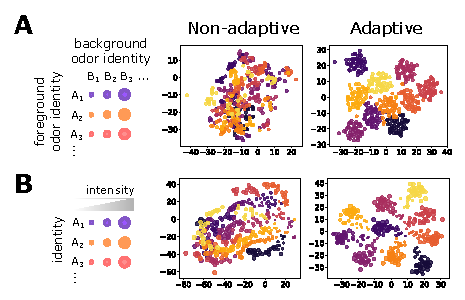
\includegraphics[width=\textwidth]{figures/2_coding_representation}
		\phantomsubcaption
		\label{fig:coding_a}
	\end{subfigure}
	\begin{subfigure}[t]{0\linewidth}
		\phantomsubcaption
		\label{fig:coding_b}
	\end{subfigure}
	\caption{\footnotesize{Front-end adaptation maintains information capacity and representations of odor identity across changes in intensity. 
    	\textbf{A}~Evolution of mutual information (MI) between odor signals and ORN response, as a function of relative odor concentration. Odor A arrives  at $t_1$ and Odor B (of similar intensity) arrives at $t_2$, where $t_2 - t_1 \gg \tau_A$. MI is plotted for both an unadaptive and adaptive system at times of order of $\tau_A$ following $t_1$ (purple; purple-blue), right before $t_2$ (blue-green), and shortly after $t_2$ (green). 
        %In a  non-adaptive system, mutual information between odor signal and ORN responses, plotted as a function of odor concentration, peaks in a regime of maximum sensitivity with the arrival of one odor (odor A), and shifts to lower concentrations with the arrival of new signals (odor B). An adaptive system pass information over a larger concentration range as ORN responses adapt, eventually  becoming un-informative over time. However, having adapted to the background, it can   then pass the information contained in subsequent signals (lower green plot).
        \textbf{B}~To investigate abstract representations of odor identity in the ORN response, ORN responses are projected from 50 dimensions to 2 dimensions, using nonlinear dimensionality reduction. In the 2D space, distinct odors are plotted as points of distinct colors, and point size represents odor intensity. 
        \textbf{C} In the adaptive system, responses cluster by identity more apparently for an adaptive system (bottom row), than a non-adaptive system (top row), shown here for 10 and 60 sparse odor identities for several concentrations each.}} % Mention that here K1 = 2, K2 = 5}}
	\label{fig:coding}
\end{figure*}

To investigate the dependence of encoding capacity on odor concentration, we calculate the mutual information (MI) between odor signals $\mathbf s$ and responses $\mathbf A$ in two sensing systems, one with ORN adaptive feedback (via Eq.~\ref{eq:adaptation_dynamics}) and one without. We consider a simple situation, in which a step of odor A, $\textbf{s}_A$,  turns on at time~$t_1$, persists for some time, and then odor B, $\mathbf s_B$ (a distinct identity) turns on at some later time~$t_2$. For simplicity, we assume that both odors have similar intensities $s_0 = \langle s_i \rangle$ and calculate the MI between the ORN responses $\mathbf {r}_a$ and signals $\mathbf s_A + \mathbf s_B$ at various times after $t_1$, as a function of $s_0$. In the non-adaptive case, MI peaks around the region of maximum sensitivity ($\sim 10^2$ a.u.) after $t_1$ (Fig.~\ref{fig:coding_a}. ORNs are firing at an elevated rate, however, more susceptible to saturation with further odor onsets. Thus, following $t_2$, the maximum shifts leftward as odors of high intensities have saturated the system and cannot pass any more information.

The adaptive system mimics the non-adaptive system at $t_1$,  before adaptation has kicked in (Fig.~\ref{fig:coding_a}). As the activity feeds back onto $\epsilon_a$, the response to higher concentrations passes through the regime of high sensitivity, and the MI peak shifts rightward. Over time, the responses for all signals have reached the baseline firing rate, and the mutual information is mostly eliminated since the firing rate is independent of odor identity. However, having now adjusted its regime of maximum sensitivity to the presence of odor A, the system can respond appropriately to odor B: the MI at $t_2$ is nearly 6 bits across 3 decades of concentration, in contrast to the non-adaptive case. These results suggest that in this multi-channel compressive system, a simple mechanism of universal integral feedback can help maintain sensitivity in changing environments.

We expect that this preservation of information capacity might therefore help maintain  abstract representations of odor identity. To examine such  representations, we project the ORN  response repertoire to a lower dimensional space using t-distributed stochastic neighbor embedding (t-SNE), a nonlinear, local dimensionality reduction technique~\cite{tsne}. Here, each data point is a 50-dimensional vector representing the ORN firing responses to a given odor of a given intensity. Each of these data points is then reduced by t-SNE to  two dimensions (Fig.~\ref{fig:coding_b}). %In Fig. 2B, colors represent odors of distinct identities; sizes represent odors of distinct concentrations. 
Testing this both for a smaller odor repertoire (10 odor identities) and a larger one (60 identities), we find that odors  separate by identity in the adaptive system, while in the unadaptive system, representations  mix among their identity and concentration (Fig.~\ref{fig:coding_b}). Together, these results suggest that at the level of ORN response, front-end adaptation helps maintain representations of odor identity across changes in odor intensity.


%%%%%%%%%%%%%%%%%%%%%%%%%%%%%%%%%%%%%%%%%%%%%%%%%%%%%%%%%%%%%%%%%
%%%%%%%%%%%%    		SIGNAL DECODING      	     %%%%%%%%%%%%
%%%%%%%%%%%%%%%%%%%%%%%%%%%%%%%%%%%%%%%%%%%%%%%%%%%%%%%%%%%%%%%%%


\subsection{Front-end adaptation promotes odor decoding and discrimination accuracy amid potential confounds}

Next, we ask how front-end adaptive mechanisms can aid in accurate signal reconstruction from a repertoire of ORN response.  One potentially complicating factor in signal reconstruction is the disparity between measurement dimension and stimulus dimension: while \textit{Drosophila} only express $\sim 60$ olfactory receptor genes~\cite{olfactory_sensory_map}, the space of aromatic odorants is far greater~\cite{vijay_1}. However, many naturally-occurring odors are comprised of only a small subset of these volatile compounds -- they are sparse in the space of odorants~\cite{vijay_1}. This is suggestive as mathematical results in compressed sensing guarantee the reconstruction of these sparse signals, assuming a sufficiently random response~\cite{CS_donoho, CS_tao, CS_ganguli}. We emphasize that while at this stage of the analysis we use a compressed sensing framework to decode these sparse signals, there is no evidence that this algorithm is being implemented in the \textit{Drosophila} olfactory circuit~\cite{chlovskii_pevlavan}. Later, we show that similar conclusions follow for odor categorization via binary and multi-class classification.

To incorporate the linear framework of compressed sensing into our nonlinear encoding model, we treat the odor encoding process exactly, while approximating the decoding to first order. Specifically, we represent the nonzero components $s_i$ of a  sparse odor mixture as $s_i = s_0 + \Delta s_i$, where $s_0$ is the center of the linearization. The target of the decoding process are the `excess' odor signal components $\Delta s_i$, which are determined by enforcing signal sparsity and the measured ORN responses through constrained optimization. The cost function to be optimized and the linear constraints are:
\begin{align}
\hat {\mathbf s} &= \text{arg min} \sum |s_i| \\
\Delta r_a &= {f}\left(\int h(\tau - t)\frac{dA_a}{ds_i}d \tau\right) \bigg |_{s_0} \Delta s_i
\end{align}
To assess the decoding performance, we denote an odor signal as accurately decoded if (i) the sparse odorant components are all estimated to within 25\% of their correct value and (ii) the components absent in the original signal (``zero" components) are all estimated as less than 10\% of the mean excess concentration, $\hat s_i \le \langle \Delta s_j \rangle$. 

%%%%%%%%%%%%%%%%%%%%%%%%%%%%%%%%%%%%%%%%%%%%%%%%%%%%%%%%%%%%%%%%%
%%%%%%%%%%%%		SIGNAL DECODING FIGURE			%%%%%%%%%%%%%
%%%%%%%%%%%%%%%%%%%%%%%%%%%%%%%%%%%%%%%%%%%%%%%%%%%%%%%%%%%%%%%%%




\begin{figure*}[!tb]
	\centering
	\begin{subfigure}[t]{\linewidth}
		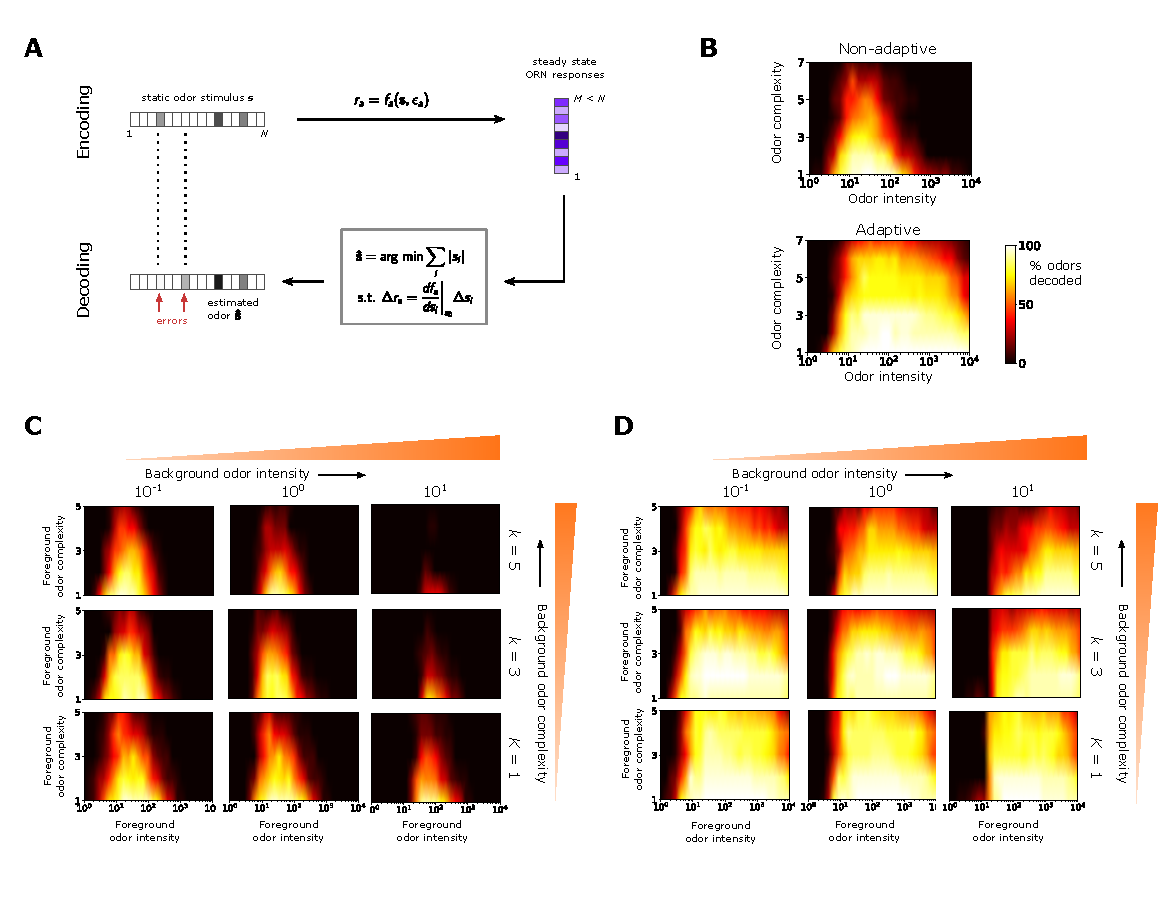
\includegraphics[width=\textwidth]{figures/3_decoding_discimination}
		\phantomsubcaption
		\label{fig:decoding_a}
	\end{subfigure}
	\begin{subfigure}[t]{0\linewidth}
		\phantomsubcaption
		\label{fig:decoding_b}
	\end{subfigure}
	\begin{subfigure}[t]{0\linewidth}
		\phantomsubcaption
		\label{fig:decoding_c}
	\end{subfigure}
	\begin{subfigure}[t]{0\linewidth}
		\phantomsubcaption
		\label{fig:decoding_d}
	\end{subfigure}
	\caption{\footnotesize{Front-end adaptation promotes accurate sparse odor decoding across concentration changes. 
    \textbf{A}~Odor stimuli produce ORN responses via odor-binding and activation and firing machinery, as described by Eqs.~\ref{eq:steady_state_act_OR}-\ref{eq:steady_state_firing}. Odors are then decoded using compressed sensing by linearizing around a background $s_0$ and minimizing the constrained $L_1$ norm of the odor signal.  Odors are assumed sparse, exhibiting $K$ nonzero components, $K \ll N$. 
    \textbf{B}~Decoding accuracy as a function of odor concentration (a.u.) and odor complexity $K$, for the non-adaptive and adaptive system respectively. 
    \textbf{C}~Decoding accuracy of foreground odors in the presence of background odors. Individual plots the decoding accuracy of the foreground as a function of its intensity and complexity, for the given background odor conditions; the intensity of the background odor increases by column and its complexity by row.
    \textbf{D}~Same as (C), for the adaptive system.}}
	\label{fig:decoding}
\end{figure*}


We apply this scheme to the ORN system described above, consisting of 50 Or/Orco complexes interacting with a 150-dimensional odorant space. We assume that number of nonzero odorants comprising the odor, $K$, is small. Note, however, that this still allows for a huge number of distinct odors, e.g. nearly 1 billion for $K= 7$. In the absence of ORN adaptation, signals are still correctly inferred in a particular regime of mean odor concentration (Fig.~\ref{fig:decoding_b}), corresponding to that of higher coding capacity in Fig.~\ref{fig:coding_a}.  Elsewhere, decoding accuracy is low. Conversely, enforcing Weber-Fechner scaling within the thresholds  $\epsilon_{\textup{L}, a}$ and $\epsilon_{\textup{H}, a}$, coding fidelity is  maintained over a several-fold change in odor intensity (Fig.~\ref{fig:decoding_b}).

In natural odor environments, accurate olfactory sensing relies on the ability to discriminate multiple odors, which may differ in chemical makeup and intensity. Even if adaptation could preserve decoding accuracy of a single odor amid intensity changes, it is conceivable that a system which adapts to average concentrations alone may well fail for multiple odors of widely differing concentrations. Accordingly,  we next consider two sparse odors, which we call the ``foreground" and ``background", and ask how well foreground odors can be decoded in the presence of backgrounds of a given intensity and molecularly complexity. In the unadaptive system, decoding accuracy in the regime of maximum sensitivity is maintained if the background concentration is low enough, but is  compromised as concentration increases (Fig.~\ref{fig:decoding_c}). For higher background concentrations, molecular complexity also has a more damaging effect on decoding accuracy. Finally, for sufficiently strong and complex background odors, the foreground is virtually undetectable (top right plot in Fig.~\ref{fig:decoding_c}). The adaptive system is substantially more robust to  backgrounds (Fig.~\ref{fig:decoding_d}), although the minimum detectable concentration increases with background intensity. Taken together, these results indicate a universal mechanism of adaptive  feedback operating on the activity of Or/Orco complexes promotes odor identification  amid potential confounds in both identity and intensity.


%%%%%%%%%%%%%%%%%%%%%%%%%%%%%%%%%%%%%%%%%%%%%%%%%%%%%%%%%%%%%%%%%
%%%%%%%%%%%%	   	   TEMPORAL CODING                %%%%%%%%%%%
%%%%%%%%%%%%%%%%%%%%%%%%%%%%%%%%%%%%%%%%%%%%%%%%%%%%%%%%%%%%%%%%%



\subsection{Odor decoding in fluctuating odor environments}
So far, we have assumed that odor signals are static in time, and that adaptation from the neural circuitry feeds back onto the receptor sensitivity instantly and perfectly. But realistic odor environments are highly intermittent and widely fluctuating, with odor concentrations that can span several orders~\cite{celani}. Further, metabolic constraints can limit adaptation speed and accuracy~\cite{ESA}. To account for temporal aspects in both the odor environment and sensing periphery, we set the timescale of adaptation in Eq.~\ref{eq:adaptation_dynamics} at $\tau_A = 250$ ms, in accordance with experimental estimates~\cite{srinivas_elife}. For simplicity, we assume that while the sensory response modulates in time, the decoding process itself is instantaneous. We also mimic a finite length of short-term memory, such that only changes in detected odor signal are remembered, and  only for up to $\tau_{\textup {F}}$ seconds in the past. If the signal is static, it will be decoded optimally between $\sim\tau_A$ and $\sim\tau_{\textup{F}}$. For fluctuating environments, we expect that $\tau_{\textup{F}}$ a few times as large as $\tau_A$ should be sufficient in detecting of whiffs of novel odors amid slowly fluctuating or static backgrounds.

%%%%%%%%%%%%%%%%%%%%%%%%%%%%%%%%%%%%%%%%%%%%%%%%%%%%%%%%%%%%%%%%%
%%%%%%%%%%%%	   	   TEMPORAL FIGURE                %%%%%%%%%%%
%%%%%%%%%%%%%%%%%%%%%%%%%%%%%%%%%%%%%%%%%%%%%%%%%%%%%%%%%%%%%%%%%



\begin{figure*}[!tb]
	\begin{subfigure}[t]{\linewidth}
		{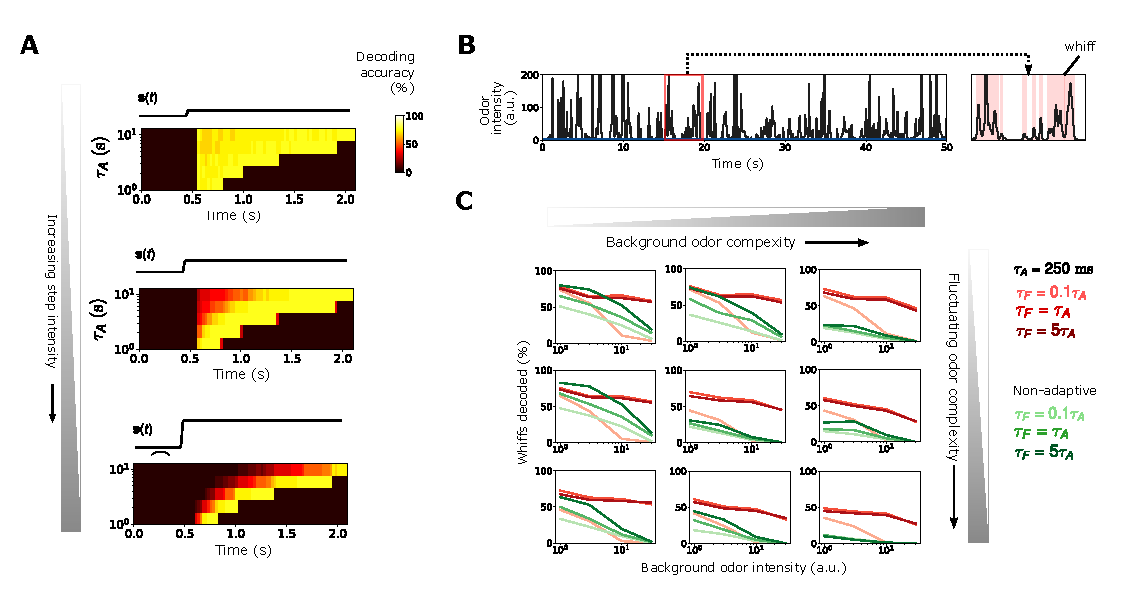
\includegraphics[width=\linewidth]{figures/4_temporal_coding}}
		\phantomsubcaption
		\label{fig:temporal_coding_a}
	\end{subfigure}
	\begin{subfigure}[t]{0\linewidth}
		\phantomsubcaption
		\label{fig:temporal_coding_b}
	\end{subfigure}
	\begin{subfigure}[t]{0\linewidth}
		\phantomsubcaption
		\label{fig:temporal_coding_c}
	\end{subfigure}
	\caption{\footnotesize{Universal ORN adaptation operating at measured timescales aids the identification of individual odor whiffs in naturalistic odor environments.
    \textbf{A}~Odor decoding accuracy before and after the onset of a step stimulus. Each plot shows the decoding accuracy in time for increasing adaptation time $\tau_A$; the plots are arranged in order of increasing step stimulus strength. 
    \textbf{B}~Naturalistic odor signal measured with photo-ionization detector downwind of a source of apple cider vinegar. Whiffs are defined as contiguous regions in which the intensity is above 10 a.u.
    \textbf{C}~Individual plots: whiff decoding accuracy as a function of background odor intensity; $\tau_A = 250$ ms in red and non-adaptive in green, light to dark for increasing $\tau_{\textup{F}}$. Rows: increasing complexity of the fluctuating odor; columns: increasing complexity of background odor. }}
	\label{fig:temporal_coding}
\end{figure*}

We first consider the simple case of step stimuli. For shallow steps, odors are rapidly decoded, though slightly more quickly for smaller $\tau_A$ (Fig.~\ref{fig:temporal_coding_a}). This is attributed the recruitment of a sufficient number of ORNs beneath the point of response saturation, such that response adaptation has little effect. For larger steps, decoding accuracy improves gradually as the system adapts at its characteristic timescale. In all cases, the accuracy drops to zero after the forgetting time $\tau_{\textup{F}}$ (here set to $4\tau_A$). 

{\color {blue} whiffs duration whiffs were not detected or not?}

We next considered a naturalistic plume, using a recorded time trace from a photo-ionization detector placed downwind of an odor source (Fig.~\ref{fig:temporal_coding_b}). The signal magnitude was scaled linearly to values applicable to our model framework (a.u.), and we verified that the plume statistics agree with theoretical predictions {~\color{blue} TODO}. %The signal is composed of a series of intermittent whiffs, defined as contiguous regions at which the concentration is above a given value. 
This signal serves as the intensity of the odor, to which we randomly assign a sparse identity from the $N$-dimensional odor space. To investigate discrimination on potentially confounding backgrounds, we add to this signal a static background odor of varying intensities and complexities, and calculate the percentage of correctly decoded odor whiffs. Without ORN adaptation, sufficiently strong backgrounds eliminate whiff-detection ability, irrespective of the complexity of either the foreground or background odor (Fig.~\ref{fig:temporal_coding_c}, green lines). In the adaptive system, this is substantially mitigated, (red lines in Fig.~\ref{fig:temporal_coding_c}) although accuracy does decrease in general with increasing background complexity. Further, accurate whiff detection requires $\tau_{\textup {F}}$ only on the order of $\tau_A$ (darker red lines). Together, this indicates that ORN adaptation acting at measured timescales  aids the detection of fluctuating odor signals amidst confounding backgrounds.

\subsection{Relationship to primacy coding hypothesis}


\begin{figure*}[!tb]
	\begin{subfigure}[t]{\linewidth}
		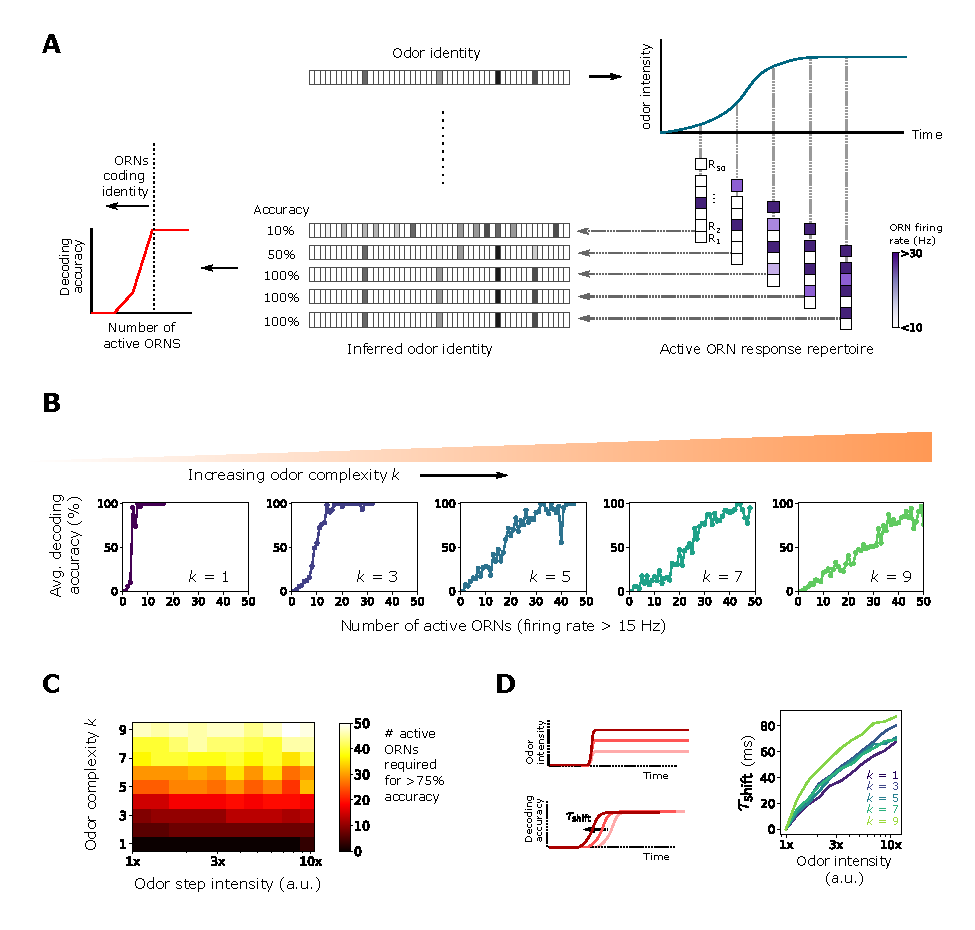
\includegraphics[width=\textwidth]{figures/5_primacy_coding}
		\phantomsubcaption
		\label{fig:primacy_coding_a}	
	\end{subfigure}
	\begin{subfigure}[t]{0\linewidth}
		\phantomsubcaption
		\label{fig:primacy_coding_b}
	\end{subfigure}
	\begin{subfigure}[t]{0\linewidth}
		\phantomsubcaption
		\label{fig:primacy_coding_c}
	\end{subfigure}
	\begin{subfigure}[t]{0\linewidth}
		\phantomsubcaption
		\label{fig:primacy_coding_d}
	\end{subfigure}
	\caption{\footnotesize{TODO}}
	\label{fig:primacy_coding}
\end{figure*}



An intriguing hypothesis emerging from recent experiments in vertebrates, ``primacy coding,"  posits that odor identity is encoded entirely by the set (but not temporal order) of the $p$ earliest responding glomeruli, known as ``primacy sets" (Fig.~\ref{fig:primacy_coding_a}). %By optogenetically masking odors at a certain point beyond the odor onset, behavioral response is completely preserved provided the mask latency  sufficiently long. Glomeruli active before mask onset are those that encode the odor identity (the primacy set), while those activating afterward confer no further information. 
Such primacy sets would in principle comprise a concentration-invariant representation of odor identity. In our framework, odors are decoded via information passed simultaneously from all 50 ORNs. However, some of this information may be redundant, whereby a set of earliest active ORNs are sufficient for odor recognition; if so, our theory would generate predictions in agreement with primacy coding. To test this, we consider a steep sigmoidal stimulus with half-max slope of $1/50$ ms$^{-1}$, as in Fig.~\ref{fig:primacy_coding_a}. We calculate the decoding accuracy as a function of time, and plot in Fig.~\ref{fig:primacy_coding_b} the accuracy as a function of number of active ORNs, which increases monotonically as the signal rises (Fig.~\ref{fig:primacy_coding_a}). To illustrate how the recruitment of ORNs incrementally improves odor signal recognition, we allow for partial accuracy by calculating  the percentage of correctly decoded individual odor components.

For sufficiently simple odors, our results are indeed in accordance with primacy coding: the set of earliest responding neurons fully account for the odor identity ($K=1, 3, 5$ plots in Fig.~\ref{fig:primacy_coding_b}). Though all ORNs eventually activate as the stimulus increases, the latter responders confer no further information in odor recognition. As expected, the active ORN subset comprising the primacy set is distinct for each odor,   {\color{blue} Show that recruited ORNs are all distinct}. We do find, however, that for more complex odor mixtures, the full ORN repertoire must be active for  accurate decoding ($K=7, 9$ plots in Fig.~\ref{fig:primacy_coding_b}), a result that holds across odor  odor concentrations (Fig.~\ref{fig:primacy_coding_c}). In this regime, there can  be no primacy code, since a primacy set consisting of the full ORN repertoire would encode only a single odor. Conversely, our framework can decode the odor for a maximal primacy set since it utilizes not just the identity of the active ORNs, but also their individual firing responses. 

Primacy sets are inherently concentration-invariant. But to what extent are they conserved among varying environmental conditions, such as persistent background odors? ORNs that have adapted their gain in response to a background odor could in principle be pushed out of the primacy sets of a novel odor due to reduced sensitivity. To test this, we calculated the primacy sets for 1000  sparse odor mixtures atop a static background of a low and high intensity. Small primacy sets finding that that primacy sets are highly conserved. This indicates that primacy coding, if true, may rely on ORN  adaptation in maintaining concentration-invariant odor representations in potentially confounding environments.




Primacy coding also predicts that for stronger stimuli, behavioral responses shift earlier in time, since the primacy set is activated quicker. We calculate this time shift and find that it rises monotonically with odor intensity over a decade of concentrations.  The timescale is on the same order as those measured (18 ms measured; here 60 ms), though the model organisms are different, so this may not be particularly meaningful. Together, these results suggest that front-end adaptation, in concert with the compressed sensing paradigm, are in partial agreement with the predictions of the primacy coding hypotheses. Our framework also provides the testable prediction that primacy coding may be limited in response to more complex odor mixtures.

\subsection{Cooperative effects of ORN adaptation and  downstream normalization}


\begin{figure*}[!tb]
	\begin{subfigure}[t]{\linewidth}
		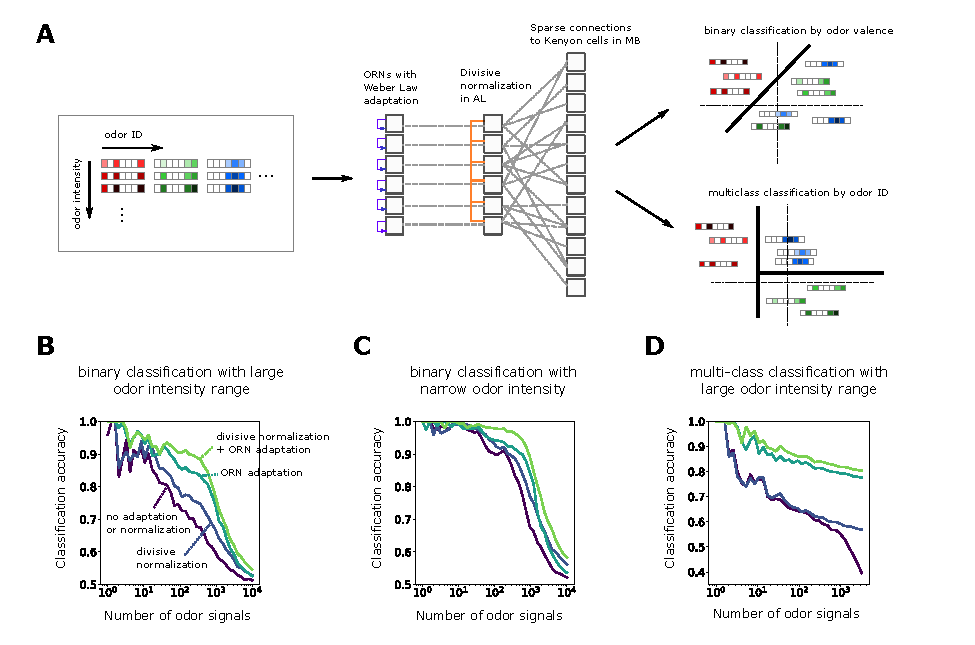
\includegraphics[width=\textwidth]{figures/6_downstream}
		\phantomsubcaption
		\label{fig:downstream_a}	
	\end{subfigure}
	\begin{subfigure}[t]{0\linewidth}
		\phantomsubcaption
		\label{fig:downstream_b}
	\end{subfigure}
	\begin{subfigure}[t]{0\linewidth}
		\phantomsubcaption
		\label{fig:downstream_c}
	\end{subfigure}
	\begin{subfigure}[t]{0\linewidth}
		\phantomsubcaption
		\label{fig:downstream_d}
	\end{subfigure}
	\caption{\footnotesize{TODO}}
	\label{fig:downstream}
\end{figure*}


Lateral inhibition among antennal lobe glomeruli normalizes ORN responses prior to their projections to the mushroom body~\cite{lateral_inh, lateral_inh_asahina}. This inhibition obeys a type of divisive gain control, normalizing each input by the sum of ORN activity~\cite{divisive_normalization}. To what extent does Weber Law adaptation in the olfactory periphery act in tandem with (or counteract) this downstream normalization to maintain odor representations? To investigate this, we extended our ORN encoding model by adding uniglomerular connections from ORNs to the antennal lobe, followed by sparse, divergent connections to 2500 Kenyon cells (KCs) in the mushroom body~\cite{memory_review, litwinkumar, abbott_axel} (Fig.~\ref{fig:downstream_a}). Divisive normalization in the AL was modeled via~\cite{divisive_normalization}:
\begin{align}
r_{\textup{PN}, a}(t) = \frac{r_a(t)^{1.5}}{\sigma^{1.5} + r_a(t)^{1.5} + (\gamma\sum_b^Mr_b(t))^{1.5}}
\end{align}
%then training and testing KC activity patterns by training
We then quantified decoding accuracy by training and testing a binary linear classifier on the KC activity output of  many sparse odors of distinct intensity and identity,  each randomly categorized as appetitive or aversive. Odor signals of the same identity but differing intensity were assigned the same valence (Fig.~\ref{fig:downstream_a}) (although, see..).  We trained the classifier on $p$ sparse odor identities at intensities chosen randomly over 4 orders of magnitude, then tested the classifier accuracy on the same odor identities but of differing concentrations. 

Classification accuracy degrades to chance level as the number of distinct odor identities $p$ becomes very high (Fig.~\ref{fig:downstream}). Either divisive normalization or ORN adaptation, when acting alone, can mitigate this, although the effect of ORN adaptation is stronger (Fig.~\ref{fig:downstream_b}). When both are active, accuracy improves further, suggesting that these distinct adaptive transformations may act jointly at different stages of neural processing to preserve representations of odor identity.  When the intensity range is narrower, overall performance improves without either adaptive mechanism at play, and their gains are mostly erased  (Fig.~\ref{fig:downstream_c}). This is expected as ... Interestingly, if we instead train the classifier to distinguish odors by their distinct identity using multiclass categorization (Fig.~\ref{fig:downstream_a}), we find that the benefits conferred by divisive normalization do not appear until $p$ is substantial, with accuracy below $65\%$ for $p \sim 50$ (Fig.~\ref{fig:downstream_d}). On the other hand, with ORN adaptation accuracy remains above $85\%$ for $p$ as high as 1000. Together, this indicates that front-end adaptation plays a key role in maintaining odor identity representations, before they are further normalized and diverged in downstream processing. In some categorization tasks, subsequent normalization can further preserve these representations.

{\color{blue} Code with temporal sequence of odors, not strength or subset? Each vector is  the sequence of temporal activation -- does adaptation help? }

%%%%%%%%%%%%%%%%%%%%%%%%%%%%%%%%%%%%%%%%%%%%%%%%%%%%%%%%%%%%%%%%%
%%%%%%%%%%%%	   	        DISCUSSION                %%%%%%%%%%%
%%%%%%%%%%%%%%%%%%%%%%%%%%%%%%%%%%%%%%%%%%%%%%%%%%%%%%%%%%%%%%%%%



\section{Discussion}

{\color {blue}-- also don't forget to mention that the odor-receptor  interactions are nonlinear and that saturation is important in this case -- also many odors}

Stopfer -- information in each pulse enough (small 50s bins) is enough to classify odors . Go further here and say that even in odor connfounds and complex odors, same conclusion follows. maybe do this for temporal presentation, not odor reconstruction, just order?

Drawing on experimental evidence for a universal mechanism of input gain control in \textit{Drosophila} olfactory receptor neurons, we propose a theoretical framework for robust, adaptive coding in dynamic odor environments. We argue that this mechanism, Weber's Law of psychophysics, plays a key role in preserving neural representations of odor identity at the front-end of the olfactory pathway, prior to further transformations downstream. Input gain control also acts jointly with normalization in the antennal lobe, implicating the importance of signal transformations at multiple steps in the circuit. We support our conclusions using both a decoding scheme that fully reconstructs odor signals from neural response, and a classification scheme that categorizes odors by identity or valence. We find that input gain control is especially central to the discrimination of fluctuating odor signals from potentially saturating odor backgrounds. For single odorants or simple odor mixtures, our results are also consistent with the primacy coding hypothesis, that signals may be fully encoded by the primacy set of earliest activating glomeruli. %Further, the primacy set is preserved even when background odors are 

\subsection{Universal front-end adaptation in multi-channel sensory systems}

In living systems, sensory adaptation ensures that responses remain in regimes of maximum sensitivity, increasing their effective dynamic range~\cite{adaptation_fairhall, adaptation_nagel, laughlin, deweese_adaptation}. Viewing sensory systems as input/output machines, the role of adaptation is therefore to maintain information capacity in dynamic environments~\cite{information_theory_adaptation}. Doing so requires matching sensory response to attributes of the environment, either by adapting to specific stimuli or to stimuli statistics~\cite{adaptation_fairhall}. In a single-channel system such as bacterial chemotaxis, information capacity is increased by matching the midpoint of the nonlinear dose-response curve, where sensitivity is highest, to mean ligand concentration~\cite{information_theory_adaptation}. This is enacted in a robust and dynamic way, through a feedback loop from the activity output of the pathway onto proteins dictating receptor sensitivity~\cite{robustness_barkai, robustness_alon}. It is hypothesized that an analogous feedback loop exists in olfactory receptor neurons, from Orco-mediated Or channel activity onto the free energy of receptor activation~\cite{srinivas_elife}. This mechanism appears to act identically across ORNs, and because olfactory receptive fields are highly overlapping, raises questions about its efficacy in complex environments: adaptation to one odor could adversely affect identification of a new odor if the latter excites some but not all of the same ORNs. Our results show that this universal mechanism of front-end gain control does help to preserve combinatorial representations of odor identity, despite these broad overlaps. 

While Weber-Fechner gain control operates at the level of individual ORNs, lateral inhibition in antennal lobe glomeruli mixes signals among all ORNs~\cite{divisive_normalization}. We find that olfactory circuits exhibiting both of these adaptive mechanisms outperform systems containing one alone. 
Combinatorial coding, therefore, benefits both from the separate adaptation of individual single sensory neurons, as well as the normalization of aggregated response. It is notable that both Weber-Fechner adaptation and divisive normalization modulate the location of maximal sensitivity rather than the scale of absolute activity -- they move dose-response curves horizontally, rather than stretching them vertically. They are both mechanisms of input gain control rather than response gain control. {\color{blue} Such input mechanisms are common to other models, sensory ssytems, etc... (...la)}. 

Other mechanisms in the sensory periphery likely play a role in maintaining neural representations of odor identity. ORNs that contain both excitatory and inhibitory responses to odorants can increase information capacity by exploiting bidirectionality of response~\cite{Cao_Tu_WL}. %Our framework uses the power law-distributed $K^*_{\textup D}$ as measured in from \textit{Drosophila} larvae, but one cannot find 
Antagonism among odorants, in which multiple odorants compete for common ORN binding sites, could effectively normalize responses provided that binding affinities and OR activation strengths are uncorrelated~\cite{reddy2017antagonism}. There, the predictions follow from a constraint on the statistics of ORN activation and binding, given that ORN activation energies are static and odor-dependent. While we rely instead on experimental evidence for dynamic gain control acting through the co-receptor Or83b, it is plausible that ion channel dynamics carry odor-specific dependencies we have not accounted for here. {\color {blue} blah..}.

\subsection{Sensing natural odor environments}

Our results are relevant for understanding combinatorial odor coding in naturalistic odor environments. Dynamic gain control acting on timescales of $\sim 250$ ms allows ORNs to more accuracy discern individual odor whiffs, particularly when such signals are mixed among static backgrounds. The gains afforded by rapid ORN adaptation increase with the strength and complexity of the background odor, suggesting that this mechanism is heavily involved in odor mixture discrimination. %Though less rare in laboratory settings, which focus on discernment of molecularly simple, static odor signals, odor discrimination is ubiquitous in the natural world. 
Indeed, {\color {blue} Add discrimination papers here}.

%\subsection{power law}


%\subsection{How to discriminate intensities?}
%Both Weber ORN adaptation and divisive gain control normalize out signal intensity, thus maintaining concentration-invariant odor representations. 

\subsection{Spatiotemporal odor coding and the primacy hypothesis}

Previous studies implicate not only the combination of active ORNs but also their distinct temporal patterns as signatures of odor identity~\cite{stopfer_temporal_model, multiple_timescales_stopfer, stopfer_nat_neuro, stopfer_temporal_channel}. ORNs modeled on observed features of these temporal patterns form distinct trajectories in low-dimensional projections, projections which cluster by odor identity, much as we have found here (Fig.~\ref{fig:coding_b}). Though we do explicitly utilize the temporal history of neural firing in our decoding schemes, the transmission of information over time is implicit in our framework. Because the strength of ORN feedback onto receptor complex activation
% $\epsilon_a(t)\tau_A = \int^t_{-\infty} dt(A_a(t) - A_{0})$, 
depends on each ORN's unique tuning curve, combinatorial ORN activity is naturally reformatted into odor- and ORN-specific patterns. The response repertoire at a given time is shaped by response history via integral feedback, and the short forgetting timescales, $\tau_{\textup F} \sim \tau_{\textup A} ~ \sim 250$ ms, suggest that only information in brief temporal windows is required for accurate odor identification, consistent with previous findings~\cite{stopfer_nat_neuro}. On the other hand, the classification scheme we employ here (Figs.~\ref{fig:downstream}) could ...



Primacy coding also exploits a unique temporal sequence of glomeruli activation, but in a coarser sense: while the order of ORN activation defines the primacy set, within this set the order is immaterial. We too find that information contained in a primacy subset of the full ORN repertoire can be sufficient for accurate reconstruction of simple odor mixtures. An interesting Primacy sets are also preserved even in the presence of potential confounds such as background odors. 




\iffalse
Coding with temporal in binary signal? -- not sure how to make linear response though.

Asahina paper
Mention mixtures
redo classification tasks with simple mixtures?
Nemenman paper
https://journals.plos.org/ploscompbiol/article?id=10.1371/journal.pcbi.1006175
\fi

%%%%%%%%%%%%%%%%%%%%%%%%%%%%%%%%%%%%%%%%%%%%%%%%%%%%%%%%%%%%%%%%%
%%%%%%%%%%%%	   	           METHODS                %%%%%%%%%%%
%%%%%%%%%%%%%%%%%%%%%%%%%%%%%%%%%%%%%%%%%%%%%%%%%%%%%%%%%%%%%%%%%




\section{Methods}

\subsection{Stochastic odor-receptor binding model}

We model an odor as an $N$-dimensional vector $\mathbf s = \langle s_1,...,s_N\rangle$, where $s_i > 0$ are the concentrations of individual volatile molecules (odorants) comprising the odor. In addition, we assume that the odors are sparse in the space of odorants, so only $K$ components of $\mathbf s$ are nonzero, where $K \ll N$. The olfactory sensory system is modeled as a collection of $M$ distinct Or/Orco complexes, each of which can be bound with any one of the odorant molecules, and can be either active (firing) inactive (quiescent). We only consider competitive binding, so a complex is bound with one odorant at most. With $N$ possible odorants, receptor $a$ resides in one of $2N+2$ possible states, \{$R_a$, $R^*_a$, $R_a$-$s_i$, $R^*_a$-$s_i$\}, indicating receptors that are unbound/inactive, unbound/active, inactive/bound to odorant $i$, and active/bound to odorant $i$, respectively. We set $N = 150$ and $M = 50$ throughout.

In the mean-field limit, the binding dynamics of these $2N + 2$ states are described by the master equations:

\begin{align}
\frac{d[R_a\text{-}s_i]}{dt} &= k^+_{ia}s_i[R_a] - k^-_{ia}[R_a\text{-}s_i] \label{eq:Meq_inactive_bind_rate}\\
\frac{d[R^*_a\text{-}s_i]}{dt} &= k^{*+}_{ia}s_i[R^*_a] - k^{*-}_{ia}[R^*_a\text{-}s_i],
\label{eq:Meq_active_bind_rate}
\end{align}
when receptor $R_a$ is either inactive (Eq.~\ref{eq:Meq_inactive_bind_rate}) or active (Eq.~\ref{eq:Meq_active_bind_rate}). Further, transitions between inactive and active states are described in the mean limit via:
\begin{align}
\frac{d[R_a]}{dt} &= w^{\text{u}+}_a [R_a] - w^{\text{u}-}_a [R^*_a] \label{eq:Meq_unbound_active_rate}\\
\frac{d[R^*_a\text{-}s_i]}{dt} &=  w^{\text{b}+}_{ia} [R_a\text{-}s_i] - w^{\text{b}-}_{ia}  [R^*_a\text{-}s_i],
\label{eq:Meq_bound_active_rate}
\end{align}
when receptor $R_a$ is either unbound (Eq.~\ref{eq:Meq_unbound_active_rate}) or bound (Eq.~\ref{eq:Meq_bound_active_rate}). The corresponding disassociation constants in terms of the binding transition rates are:


\begin{align}
K_{ia} = \frac{k^-_{ia}}{k^+_{ia}} \nonumber \\
K^*_{ia} = \frac{k^{*-}_{ia}}{k^{+*}_{ia}} 
\label{eq:Kd}
\end{align}

Following~\cite{srinivas_elife}, we assume that in steady state, the active firing state of an Or/Orco complex is energetically suppressed from the inactive state through corresponding Boltzmann factors:

\begin{align}
\frac{[R^*_a]}{[R_a]} &= \frac{w^{\text{u}+}_a}{w^{\text{u}-}_a} \equiv e^{-\epsilon_a} \label{eq:epsilon_unbound} \\
\frac{[R^*_a\text{-}s_i]}{[R_a\text{-}s_i]} &= \frac{w^{\text{b}+}_{ia}}{w^{\text{b}-}_{ia}} \equiv e^{-\epsilon^{\text b}_{ia}}.\label{eq:epsilon_bound}
\end{align}
These energies are related through detailed balance, which we assume. Applying detailed balance to a given 4-cycle 
\begin{align}
R_a \rightarrow R_a^* \rightarrow R_a^*\text{-}s_i \rightarrow R_a\text{-}s_i \rightarrow R_a
\end{align}
gives
\begin{align}
\frac{w^{\text{u}+}_a}{w^{\text{u}-}_a}\frac{k^{*+}_{ia}}{k^{*-}_{ia}}\frac{w^{\text{b}-}_{ia}}{w^{\text{b}+}_{ia}}\frac{k^{-}_{ia}}{k^{+}_{ia}} \equiv 1,
\label{eq:detailed_balance}
\end{align}
which, in conjunction with Eqs.~\ref{eq:Kd}, \ref{eq:epsilon_unbound}, and \ref{eq:epsilon_bound}, gives
\begin{align}
\epsilon_{ia}^{\text b} = \epsilon_a + \ln\left[\frac{K^*_{ia}}{K_{ia}}\right].
\label{testing_equation}
\end{align}
Assuming the binding dynamics are fast, then the probability that receptor $a$ is bound by ligand~$i$ when inactive and active can be derived from  Eqs.~\ref{eq:Meq_inactive_bind_rate} and \ref{eq:Meq_active_bind_rate} as
\begin{align}
p^{\text b}_{ia} = \frac{s_i/K_{ia}}{1 + \sum_j^Ns_j/K_{ja}} \label{eq:bound_prob_ai_inactive} \\
p^{\text b, *}_{ia} = \frac{s_i/K^*_{ia}}{1 + \sum_j^Ns_j/K^*_{ja}} \label{eq:bound_prob_ai_active}.
\end{align}
The average  activity $A_a$ of complex $a$ is the likelihood that the complex is active, unbound or unbound (equivalantly, the proportion of Or/Orco complexes in a given ORN that are active):
\begin{align}
A_a = \frac{[R^*_a] + \sum_i^N[R^*_a\text{-}s_i]}{[R^*_a] + \sum_i^N[R^*_a\text{-}s_i] + {[R_a] + \sum_i^N[R_a\text{-}s_i]}}.
\end{align} 
Using the master equations between active and inactive states Eq.~\ref{eq:Meq_unbound_active_rate} and \ref{eq:Meq_bound_active_rate}, this activity obeys the master equation
\begin{align}
\frac{dA_a}{dt} &= w^+_a(1 - A_a) + w^-_aA_a
\label{eq:dadt}
\end{align}
with effective transition rates
\begin{align}
w^+_a &= \sum_i^Np^{\text b}_{ia} w^{\text u +}_{ia} + p_{a}w^{\text u}_a 
\end{align}
and analogously for $w_a^-$. Setting Eq.~\ref{eq:dadt} to zero gives the steady state average activity level of ORN $a$:
\begin{align}
A_a = \left(1 + e^{\epsilon_a}\frac{1 + \sum_i^N s_i/K_{ia}}{1 + \sum_i^N s_i/K^*_{ia}}\right)^{-1}. \tag{\ref{eq:steady_state_act}}
\end{align}
	
\subsection{Generation of binding matrices $K^*_{ia}$}
 TODO

\subsection{Compressed sensing decoding of ORN response}
We decode ORN responses to infer odor signal identities using an abstraction intended to mimic the neural computations underlying odor identification in the \textit{Drosophila} mushroom body. While we make no assumptions that the compressed sensing (CS) algorithm (or one like it) is being utilized in actuality, this framework nonetheless informs our understanding of how the neural representation of odor identity is maintained or lost when passed through a distributed ORN repertoire. In this sense, CS is somewhat of an upper bound on how well a real neural computation might perform in decompressing ORN responses.

We assume that ORN firing rates are linear in the Or/Orco complex activity; for simplicity we let this transform be the identity. Though subsequent neural circuitry, particularly from the glomeruli in the AL to the Kenyon cells in the MB further mix and scramble these responses, we focus here on the information transfer at the sensory periphery alone. In any case, as demonstrated previously~\cite{vijay_1}, we expect that these neural computations would only improve the representation of neural identity, so we expect no negative ramifications for our findings.

CS addresses the problem of determining a sparse signal from a set of linear measurements, when the number of measurements is less than the signal dimension. Specifically, it is a solution to 
\begin{align}
\mathbf y = \mathbf R\mathbf s,
\label{eq:CS_constraints}
\end{align} where $\mathbf s \in \mathbb{R}^N$ and $\mathbf a\in \mathbb{R}^M$ are vectors of signals and responses, respectively, and $\mathbf R$ is the measurement matrix. Since measurements are fewer than signal components, then $M < N$, whereby $\mathbf R$ is wide rectangular and so Eq.~\ref{eq:CS_constraints} cannot be simply inverted to produce $\mathbf s$. The idea of CS is to utilize the knowledge that $\mathbf s$ is sparse, i.e.g only $K$ of its components, $K \ll N$ are nonzero. Both the measurements and sparsity are thus combined into a single constrained optimization routine:
\begin{align}
\hat s_i = \textup{argmin} \sum_i^N |s_i| \quad \textup{such that } \mathbf y = \mathbf R\mathbf s
\label{eq:CS}
\end{align}
where $\hat s_i$ are the optimal estimates of the signal components and the sum, which is known as the $L_1$ norm of $\mathbf s$, is a natural metric of sparsity. 

Importantly, the $L_1$ norm is a convex operation and the constraints are linear, so the optimization has a unique global minimum. To incorporate the nonlinear response of our encoding model into this linear framework, we assume that the responses are generated through the full nonlinear steady state response, Eq.~\ref{eq:steady_state_act}, but that the measurement matrix needed for decoding uses a linear approximation of this transformation.  Expanding Eq.~\ref{eq:steady_state_act} around $s_0 = s_i - \Delta s_i$ gives
\begin{align}
A_a &\approx A_{a, 0} + \Delta A_a \label{eq:CS_act_approx} \\
\Delta A_a &= \sum_i^NR_{ia}\big|_{s_0}\Delta s_i \label{eq:CS_dAct_approx}\\
A_{a, 0} &= \frac{\sum_1^N s_0/K_{ia}^*}{\sum_1^N s_0/K_{ia}^* + e^{\epsilon_a}} \label{eq:CS_act0_approx} \\
R_{ia}\big|_{s_0} &=  \frac{e^{\epsilon_a}/K_{ia}^*}{(\sum_i^Ns_0/K_{ia}^* + e^{\epsilon_a})^2},
\label{eq:CS_gain_approx}
\end{align}
where we work in the approximation $K^*_{ia} \ll~s_0 \ll K_{ia}$. We assume that the neural system has access to the linearized response, Eq.~\ref{eq:CS_gain_approx}, but must infer the excess signals $\Delta s_i$ from the excess activity $\Delta A_a$. Corresponding to the CS framework, therefore, $\Delta \mathbf {A} \rightarrow \mathbf y$, $\Delta \mathbf s \rightarrow \mathbf s$, and $R_{ia}\big|_{s_0} \rightarrow \mathbf R$. We optimize the cost function in Eq.~\ref{eq:CS} using sequential least squares programming, implemented in Python through using the scientific package SciPy.

\subsection{Or/Orco  energies of activation $\epsilon_a$ and enforcement of Weber's Law}
Free energies are considered receptor-independent throughout, with the exception of dynamically adaptive system in a temporal odor environment (Figs.~\ref{fig:temporal_coding} and \ref{fig:temporal_coding_2}). To enforce Weber's Law, we assume the receptor activities feed back onto $\epsilon_a$ through the free energies. For the static case, adaptation is perfect, whereby Or/Orco activities are pegged to perfectly adapted values $\bar {A}_{a}$. Incorporating this into Eq.~\ref{eq:steady_state_act}, and assuming  $K^*_{ia} \ll s \ll K_{ia}$, gives
\begin{align}
\bar \epsilon_a &= \ln\left(\frac{1-\bar {A}_{a}}{\bar {A}_{a}}\right) + \ln\left(\sum_i^N\frac{s_i}{K_{ia}^*}\right).
\label{eq:adapted_epsilon}
\end{align}
Assuming that the excess signals are small, $\Delta s_i < s_0$, this gives 
\begin{align}
\epsilon_a \approx \ln(s_0) + \epsilon_{a, 0},
\label{eq:WL_approx}
\end{align} 
where $\epsilon_{a, 0}$ are receptor-dependent constants. In the static case, we choose these constants such that $\epsilon_{a}$ in both adaptive and non-adaptive systems are equivalent, equal to $\epsilon_{\text {L}}$, at a given low concentration, $s_{0, \text L}$.  Below this concentration, we assume adaptation is not in effect, so $\epsilon_a  = \epsilon_{\text {L}}$.  

It is important to note that while the linearized gain Eq.~\ref{eq:CS_gain_approx} utilized by the decoding algorithm appears to rely on $\epsilon_a$, by the above argument $\epsilon_a$ can in principle be determined by firing rates alone. That is, $\epsilon_a$ is inferred in time through integration of Eq.~\ref{eq:WL_dynamics}, which relies only on the current ORN activity.


\begin{table*}[!tb]
	\centering
	{\small
		\begin{tabular}{ccccccccccccccc}
			Figure & $N$& $M$ & $K$ & $\mu_{a, \text L}$ & $\mu_{a, \text H}$ & $\nu_{a, \text L}$ & $\nu_{a, \text H}$ & $\epsilon_{a, 0}$ & $\epsilon_{\text {L}}$  & $\epsilon_{\text {H}}$  & $s_{0, \text L}$ & $s_k$ & $s_{k, \text F}$\\[0.1cm]
			
			\hline \\[-0.2cm]
			\smallskip
			
			\ref{fig:tuning_curves_c} & 200 & 40 & 6 & $2\cdot 10^{-4}$ & $10^{-3}$ & $10^{-2}$ & 1.0 & 5.4 & 5.4 & 10  & - & $ \mathcal N\left(\frac{s_0}{5}, \frac{s_0}{15}\right)$ & --\\
			
			\ref{fig:decoding_a} & 100 & 50 & 7 & 0.5 & 0.5 & 0.8 & 0.8 & 5.4 & 3.1 & 10  & $10^{-1}$ & $ \mathcal N\left(\frac{s_0}{3}, \frac{s_0}{15}\right)$ & -- \\
			
			\ref{fig:decoding_b} & 100 & 50 & 7 & 0.5 & 0.6 & 0.6 & 0.9 & 5.4 & 3.1 & 10 & $10^{-1}$ & $ \mathcal N\left(\frac{s_0}{3}, \frac{s_0}{15}\right)$ & ---\\
			
			\ref{fig:decoding_c} & 100 & 50 & 7 & 0.5 & 0.6 & 0.6 & 0.9 & 5.4 & 3.1 & 10 & $10^{-1}$ & $ \mathcal N\left(\frac{s_0}{3}, \frac{s_0}{15}\right)$ & -- \\
			
			\ref{fig:signal_discrimination_a}-\ref{fig:signal_discrimination_h} & 100 & 50 & 7 & 0.5 & 0.6 & 0.6 & 0.9 & 5.4 & 3.1 & 10 & $10^{-1}$ & $ \mathcal N\left(\frac{s_0}{3}, \frac{s_0}{15}\right)$ & $ \mathcal N(1, \frac{1}{5})$ \\
			
			\ref{fig:temporal_coding} & 100 & 50 & 7 & 0.5 & 0.6 & 0.6 & 0.9 & -- & -- & -- & $10^{-2}$ & $ \mathcal N\left(\frac{s_0}{3}, \frac{s_0}{9}\right)$ & -- \\
			
			\ref{fig:temporal_coding_2} & 100 & 50 & 7 & 0.5 & 0.6 & 0.6 & 0.9 & -- & -- & -- & $10^{-2}$ & $ \mathcal N\left(\frac{s_0}{3}, \frac{s_0}{9}\right)$ & -- \\
		\end{tabular}
	}
	\caption{Parameters for simulations in all of the figures.}
	\label{tab:params}
\end{table*}



\subsection{Odor signals}
Odor signals $\mathbf s$ are $N$-dimensional vectors presumed sparse whereby only $K$ components, $s_k$ are nonzero,  $K~\ll~N$. The magnitudes of the nonzero components $s_k$ are denoted $s_0 + \Delta s_k$. Here, $\Delta s_k$ is a random vector, while $s_0$ is both the center of linearization and, in the case of the adaptive system, the value dictating the strength of adaptive feedback $\epsilon_a\sim\ln\langle s_0 \rangle$. 

All the signal intensities are in arbitrary units, as they can be scaled to any range by a corresponding shift in the scales of $K_{ia}$ and $K^*_{ia}$.

\subsection{Dynamic adaptation}

Dynamic adaptation is enforced through
\begin{align}
	\frac{d\epsilon_a(t)}{dt} &= \frac{1}{\tau_a}\left[A_a - \bar {A}_{a}\right].
	\tag{\ref{eq:WL_dynamics}}
\end{align}
The perfectly adapted activity levels $\bar {A}_{a}$ are determined by evaluating Eq.~\ref{eq:steady_state_act} at a given odor intensity, $s_{0, \text{L}}$, corresponding to a minimum stimulus at which adaptation takes effect. The decoding step is assumed instantaneous, so decoded odor identity $\mathbf {\hat s}$ is determined by the current value of $\epsilon_a$ (which, by virtue of Eq.~\ref{eq:WL_dynamics}, is determined by ORN activity a short time prior).

For the simulations with two fluctuating odors (Figs.~\ref{fig:temporal_coding_2}), the traces shown correspond to the values of $s_0$ (in blue) and $s_{0, \text{b}}$ (orange), where $s_{0, \text{b}}$ is the baseline concentration of the background odor components, to which the excess signals $\Delta s_{k, \text {b}}$ are added to set the individual odorant concentrations. We choose $\Delta s_{k, \text {b}}~\sim~\mathcal N(s_{k, \text {b}}/3, s_{k, \text {b}}/9)$.

\subsection{Parameter values used in all figures}

Parameter values for all of the plots are listed in Table~\ref{tab:params}.
